\documentclass{standalone}
\usepackage{tikz}
\usetikzlibrary{patterns, positioning}
\usepackage[sfdefault]{ClearSans} %% option 'sfdefault' activates Clear Sans as the default text font
\usepackage[T1]{fontenc}

\begin{document}
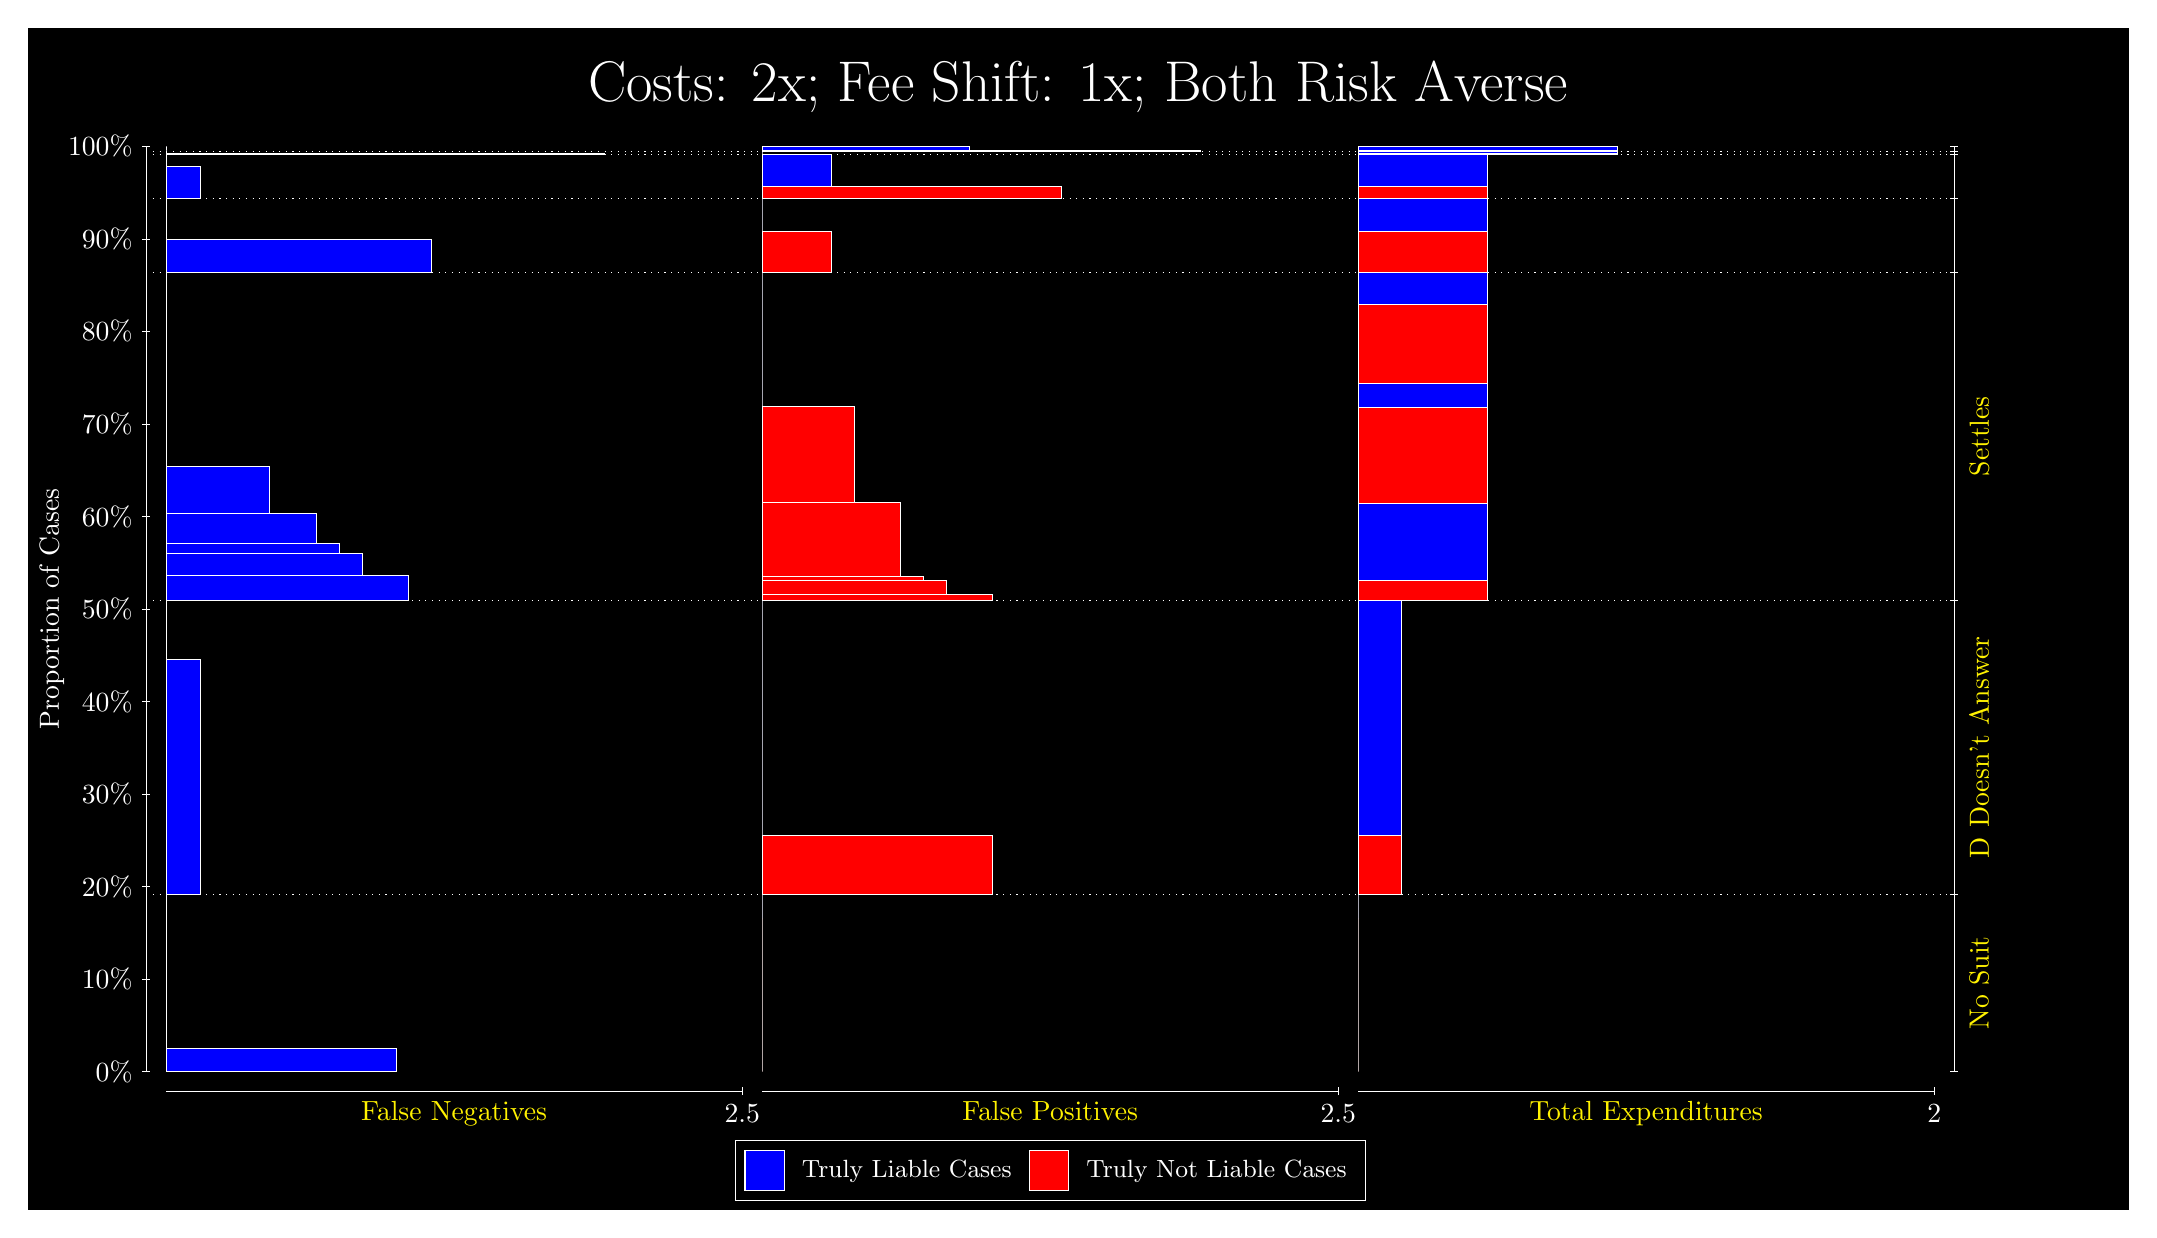
\begin{tikzpicture}
\draw[fill=black] (0,0) rectangle (26.667,15);
\draw[text=white] (0,13.5) rectangle (26.667,15) node[midway] {\huge Costs: 2x; Fee Shift: 1x; Both Risk Averse};
\draw[white, very thin] (1.5,1.75) -- (1.5,13.5);
\node[rotate=90, text=white, anchor=center] at (0.3, 7.625) {Proportion of Cases};
\draw[white, very thin] (1.45,1.75) -- (1.55,1.75);
\node[text=white, anchor=east] at (1.45, 1.75) {0\%};
\draw[white, very thin] (1.45,2.925) -- (1.55,2.925);
\node[text=white, anchor=east] at (1.45, 2.925) {10\%};
\draw[white, very thin] (1.45,4.1) -- (1.55,4.1);
\node[text=white, anchor=east] at (1.45, 4.1) {20\%};
\draw[white, very thin] (1.45,5.275) -- (1.55,5.275);
\node[text=white, anchor=east] at (1.45, 5.275) {30\%};
\draw[white, very thin] (1.45,6.45) -- (1.55,6.45);
\node[text=white, anchor=east] at (1.45, 6.45) {40\%};
\draw[white, very thin] (1.45,7.625) -- (1.55,7.625);
\node[text=white, anchor=east] at (1.45, 7.625) {50\%};
\draw[white, very thin] (1.45,8.8) -- (1.55,8.8);
\node[text=white, anchor=east] at (1.45, 8.8) {60\%};
\draw[white, very thin] (1.45,9.975) -- (1.55,9.975);
\node[text=white, anchor=east] at (1.45, 9.975) {70\%};
\draw[white, very thin] (1.45,11.15) -- (1.55,11.15);
\node[text=white, anchor=east] at (1.45, 11.15) {80\%};
\draw[white, very thin] (1.45,12.325) -- (1.55,12.325);
\node[text=white, anchor=east] at (1.45, 12.325) {90\%};
\draw[white, very thin] (1.45,13.5) -- (1.55,13.5);
\node[text=white, anchor=east] at (1.45, 13.5) {100\%};

\draw[white, very thin] (24.457,1.75) -- (24.457,13.5);
\draw[white, very thin] (24.407,1.75) -- (24.507,1.75);
\node[anchor=west] at (24.407, 1.75) {};
\draw[white, very thin] (24.407,3.9982) -- (24.507,3.9982);
\node[anchor=west] at (24.407, 3.9982) {};
\draw[white, very thin] (24.407,7.7356) -- (24.507,7.7356);
\node[anchor=west] at (24.407, 7.7356) {};
\draw[white, very thin] (24.407,11.901) -- (24.507,11.901);
\node[anchor=west] at (24.407, 11.901) {};
\draw[white, very thin] (24.407,12.841) -- (24.507,12.841);
\node[anchor=west] at (24.407, 12.841) {};
\draw[white, very thin] (24.407,13.4) -- (24.507,13.4);
\node[anchor=west] at (24.407, 13.4) {};
\draw[white, very thin] (24.407,13.433) -- (24.507,13.433);
\node[anchor=west] at (24.407, 13.433) {};
\draw[white, very thin] (24.407,13.5) -- (24.507,13.5);
\node[anchor=west] at (24.407, 13.5) {};

\draw[white, very thin, fill=blue] (1.75,1.75) rectangle (4.6775,2.0492);
\draw[white, very thin, fill=red] (1.75,2.0492) rectangle (1.75,3.9982);
\draw[white, very thin, fill=blue] (1.75,3.9982) rectangle (2.1891,6.9835);
\draw[white, very thin, fill=red] (1.75,6.9835) rectangle (1.75,7.7356);
\draw[white, very thin, fill=blue] (1.75,7.7356) rectangle (4.8239,8.0512);
\draw[white, very thin, fill=blue] (1.75,8.0512) rectangle (4.2384,8.3337);
\draw[white, very thin, fill=blue] (1.75,8.3337) rectangle (3.9457,8.4613);
\draw[white, very thin, fill=blue] (1.75,8.4613) rectangle (3.6529,8.8435);
\draw[white, very thin, fill=blue] (1.75,8.8435) rectangle (3.0674,9.4376);
\draw[white, very thin, fill=red] (1.75,9.4376) rectangle (1.75,11.901);
\draw[white, very thin, fill=blue] (1.75,11.901) rectangle (5.1167,12.318);
\draw[white, very thin, fill=red] (1.75,12.318) rectangle (1.75,12.841);
\draw[white, very thin, fill=blue] (1.75,12.841) rectangle (2.1891,13.247);
\draw[white, very thin, fill=red] (1.75,13.247) rectangle (1.75,13.4);
\draw[white, very thin, fill=blue] (1.75,13.4) rectangle (7.3123,13.415);
\draw[white, very thin, fill=red] (1.75,13.415) rectangle (1.75,13.433);
\draw[white, very thin, fill=red] (1.75,13.433) rectangle (1.75,13.449);
\draw[white, very thin, fill=blue] (1.75,13.449) rectangle (1.75,13.5);
\draw[white, very thin, fill=red] (9.3189,1.75) rectangle (9.3189,3.699);
\draw[white, very thin, fill=blue] (9.3189,3.699) rectangle (9.3189,3.9982);
\draw[white, very thin, fill=red] (9.3189,3.9982) rectangle (12.246,4.7503);
\draw[white, very thin, fill=blue] (9.3189,4.7503) rectangle (9.3189,7.7356);
\draw[white, very thin, fill=red] (9.3189,7.7356) rectangle (12.246,7.8061);
\draw[white, very thin, fill=red] (9.3189,7.8061) rectangle (11.661,7.9901);
\draw[white, very thin, fill=red] (9.3189,7.9901) rectangle (11.368,8.0346);
\draw[white, very thin, fill=red] (9.3189,8.0346) rectangle (11.075,8.9854);
\draw[white, very thin, fill=red] (9.3189,8.9854) rectangle (10.49,10.199);
\draw[white, very thin, fill=blue] (9.3189,10.199) rectangle (9.3189,11.901);
\draw[white, very thin, fill=red] (9.3189,11.901) rectangle (10.197,12.425);
\draw[white, very thin, fill=blue] (9.3189,12.425) rectangle (9.3189,12.841);
\draw[white, very thin, fill=red] (9.3189,12.841) rectangle (13.125,12.995);
\draw[white, very thin, fill=blue] (9.3189,12.995) rectangle (10.197,13.4);
\draw[white, very thin, fill=red] (9.3189,13.4) rectangle (9.3189,13.418);
\draw[white, very thin, fill=blue] (9.3189,13.418) rectangle (9.3189,13.433);
\draw[white, very thin, fill=red] (9.3189,13.433) rectangle (14.881,13.449);
\draw[white, very thin, fill=blue] (9.3189,13.449) rectangle (11.954,13.5);
\draw[white, very thin, fill=red] (16.888,1.75) rectangle (16.888,3.699);
\draw[white, very thin, fill=blue] (16.888,3.699) rectangle (16.888,3.9982);
\draw[white, very thin, fill=red] (16.888,3.9982) rectangle (17.437,4.7503);
\draw[white, very thin, fill=blue] (16.888,4.7503) rectangle (17.437,7.7356);
\draw[white, very thin, fill=red] (16.888,7.7356) rectangle (18.534,7.9901);
\draw[white, very thin, fill=blue] (16.888,7.9901) rectangle (18.534,8.9664);
\draw[white, very thin, fill=red] (16.888,8.9664) rectangle (18.534,10.18);
\draw[white, very thin, fill=blue] (16.888,10.18) rectangle (18.534,10.496);
\draw[white, very thin, fill=red] (16.888,10.496) rectangle (18.534,11.491);
\draw[white, very thin, fill=blue] (16.888,11.491) rectangle (18.534,11.901);
\draw[white, very thin, fill=red] (16.888,11.901) rectangle (18.534,12.425);
\draw[white, very thin, fill=blue] (16.888,12.425) rectangle (18.534,12.841);
\draw[white, very thin, fill=red] (16.888,12.841) rectangle (18.534,12.995);
\draw[white, very thin, fill=blue] (16.888,12.995) rectangle (18.534,13.4);
\draw[white, very thin, fill=red] (16.888,13.4) rectangle (20.181,13.418);
\draw[white, very thin, fill=blue] (16.888,13.418) rectangle (20.181,13.433);
\draw[white, very thin, fill=red] (16.888,13.433) rectangle (20.181,13.449);
\draw[white, very thin, fill=blue] (16.888,13.449) rectangle (20.181,13.5);
\draw[white, dotted] (1.5,3.9982) -- (24.457,3.9982);
\draw[white, dotted] (1.5,7.7356) -- (24.457,7.7356);
\draw[white, dotted] (1.5,11.901) -- (24.457,11.901);
\draw[white, dotted] (1.5,12.841) -- (24.457,12.841);
\draw[white, dotted] (1.5,13.4) -- (24.457,13.4);
\draw[white, dotted] (1.5,13.433) -- (24.457,13.433);
\draw[white, very thin] (1.75,1.5) -- (9.0689,1.5);
\node[text=yellow, anchor=north] at (5.4094, 1.5) {False Negatives};
\draw[white, very thin] (9.0689,1.45) -- (9.0689,1.55);
\node[text=white, anchor=north] at (9.0689, 1.45) {2.5};

\draw[white, very thin] (9.3189,1.5) -- (16.638,1.5);
\node[text=yellow, anchor=north] at (12.978, 1.5) {False Positives};
\draw[white, very thin] (16.638,1.45) -- (16.638,1.55);
\node[text=white, anchor=north] at (16.638, 1.45) {2.5};

\draw[white, very thin] (16.888,1.5) -- (24.207,1.5);
\node[text=yellow, anchor=north] at (20.547, 1.5) {Total Expenditures};
\draw[white, very thin] (24.207,1.45) -- (24.207,1.55);
\node[text=white, anchor=north] at (24.207, 1.45) {2};

\node[text=yellow, centered, rotate=90] at (24.777, 2.8741) {No Suit};
\node[text=yellow, centered, rotate=90] at (24.777, 5.8669) {D Doesn't Answer};
\node[text=yellow, centered, rotate=90] at (24.777, 9.8183) {Settles};





\draw (12.978300999999998,1.5) node[draw=none] (baseCoordinate) {};
\begin{scope}[align=center]
        \matrix[scale=0.5, draw=white, below=0.5cm of baseCoordinate, nodes={draw}, column sep=0.1cm]{
            \node[rectangle, draw, minimum width=0.5cm, minimum height=0.5cm, fill=blue] {}; &
            \node[draw=none, font=\small, text=white] (B) {Truly Liable Cases}; &
            \node[rectangle, draw, minimum width=0.5cm, minimum height=0.5cm, fill=red] {}; &
            \node[draw=none, font=\small, text=white] (B) {Truly Not Liable Cases}; \\
            };
\end{scope}

\end{tikzpicture}
\end{document}